\section{Runtime cost comparison on a real-world MeerKAT reconstruction}\label{scale}
Current Compressed Sensing reconstructions produce images at a higher quality than CLEAN. However, CLEAN is significantly cheaper to compute. MeerKAT's large scale reconstruction problems, CLEAN is still the go-to algorithm. In this project, we developed for a new architecture, which uses the relevant columns of the Fourier Transform Matrix directly. We developed a Coordinate Descent algorithm with this architecture and demonstrated in section \ref{results} super-resolution performance on simulated data. The question, if we can lower the runtime costs with our new architecture, is still open. 

In this section, we compare the costs of Coordinate Descent with WSCLEAN, which is the reconstruction algorithm of choice for MeerKAT reconstructions. We create cost functions for each algorithm, which estimate the number of operations depending on the input size. WSCLEAN was executed on a real-world MeerKAT dataset shown in image \ref{scale:wsclean}. Our proof-of-concept implementation was not able to handle the large amount of data. Instead, we extrapolate the best-case costs of our approach and compare them to WSCLEAN on the MeerKAT dataset.


\subsection{Cost function of an idealized Coordinate Descent}
The runtime cost of Coordinate Descent depends on the number of Visibilities $M$ and the number of non-zero starlets $S$. The number and location of the $S$ non-zero starlets are generally not known. However, we created a heuristic which finds likely non-zero starlet components. In a realistic setting, the heuristic will have found more than $S$ likely non-zero starlets. For the idealized version of Coordinate Descent, we assume an oracle performance heuristic: It finds the location and number of the $S$ non-zero starlet components in constant time. Coordinate Descent therefore has to calculate the value of $S$  components. In total, the idealized Coordinate Descent algorithm uses four steps: creating $J$ starlet levels with the non-uniform FFT, creating the columns of $F^{-1}$, calculating the minima for each single component, and calculating the starlet layers:

\begin{alignat*}{1}
J \text{non-uniform FFTs for the starlet regularization} &: J*(M + 2N*ld(2N))\\
\text{creating} \:S\: \text{columns of}\: F^{-1} &: S*7M\\
\text{locating} \:S\: \text{minima of} \:S\: \text{parabolas} &: S*4M\\
\text{calculating} \:J\: \text{Starlet layers} &: J * 2M
\end{alignat*}

We assume we have enough memory to cache the columns of $F^{-1}$ and only need to calculate them once. Keep in mind that each column of $F^{1}$ has the same length as the Visibilities, essentially multiplying the input data. The last parameter for Coordinate Descent is the number of iterations to converge, $I_CD$. Estimating this number is difficult as Coordinate Descent does not have strict guarantees (as discussed in section \ref{cd}). Instead, we assume it converges after a fixed number of iterations. Therefore we arrive at the cost function of \eqref{results:cd:omega}.

\begin{equation}\label{results:cd:omega}
\begin{aligned}
	CD(I_{CD}, M, S, J) = &I_{CD} * [S * 4M + J * 2M]\\
		&+  S*7M\\
		&+ J*(M + 2N*ld(2N))
\end{aligned}
\end{equation}

Note that the runtime of Coordinate Descent is independent of the number of pixels. The only image related parameter in \eqref{results:cd:omega} is $J$, the number of starlet layers. The largest starlet layer represents the largest possible structure in the image, which is given by the instrument and the image resolution. The runtime only depends indirectly on the image resolution, not the total number of pixels. For simplicity, we assume the image cannot have structures larger than half the image size. For our MeerKAT example, this is more than enough to represent the largest structures.

Also note the term iterating over the $S$ non-zero starlets, $ I_{CD} * [S * 4M +\ldots]$. As it turns out, this is the Achilles heel of the algorithm. MeerKAT observations contain a very large amount of Visibilities $M$.

\subsection{Cost function of WSCLEAN}
The WSCLEAN algorithm uses the Major Cycle architecture. It uses the non-uniform FFT with $w$-stacking. The runtime costs of a single Major Cycle depends on the non-uniform FFT with $w$-stacking and the number of CLEAN deconvolutions. $N$ denotes the number of pixels.

\begin{alignat*}{1}
	\text{non-uniform FFT} &: M + 2N*ld(2N)\\
	\text{non-uniform FFT with} \:w\text{-stacking} &:M + W*(2N*ld(2N) + 2N) + N*ld(N)\\
	I_{WSCLEAN}\: \text{deconvolutions} &: I_{WSCLEAN}*2N
\end{alignat*}

The overall cost function shown in \eqref{results:clean:o} can also be split into two parts. In each Major Cycle, the forward and backwards non-uniform FFTs gets calculated, and CLEAN deconvolves the image for a certain number of iterations.

\begin{equation}\label{results:clean:o}
\begin{aligned}
 WSCLEAN(I_{Major}, I_{CLEAN}, M, N,  W) =\: &I_{Major} * 2 * [M + W*(2N*ld(2N) + 2N) + N log N]\\
	&+ I_{Major} * [I_{CLEAN}*2N]
\end{aligned}
\end{equation}

Notice that the number of CLEAN deconvolutions $I_{CLEAN}$ depends on the image content, similar the number of non-zero starlets $S$ for Coordinate Descent. Here however, it multiplies with the number of pixels instead of the number of Visibilities. In a sense, the major cycle tries to reduce the runtime complexity of handling the image content by calculating the non-uniform FFT. If the difference is large enough $N \ll M$, then the Major Cycle will end up with a smaller runtime costs.


\subsection{Comparison on a MeerKAT reconstruction problem}
Our real-world MeerKAT observation has been calibrated and averaged in frequency and time to reduce storage space. The resulting dataset contains 540 channels with 4 million Visibilities each. Due to hardware limitations, WSCLEAN was calculated on 75 channels. The reconstructed image is shown in \ref{scale:wsclean}, and the resulting parameters for our cost function are: 
\begin{itemize}
	\item Major Cycles: $I_{Major} = 6$
	\item Number of CLEAN iterations: $I_{CLEAN} = 35'000$
	\item Visibilities: $M=3.05e^8$
		\item Pixels: $N = 2048^2$
	\item $w$-stacks: $W = 32$
\end{itemize}

\begin{figure}[h]
	\centering
	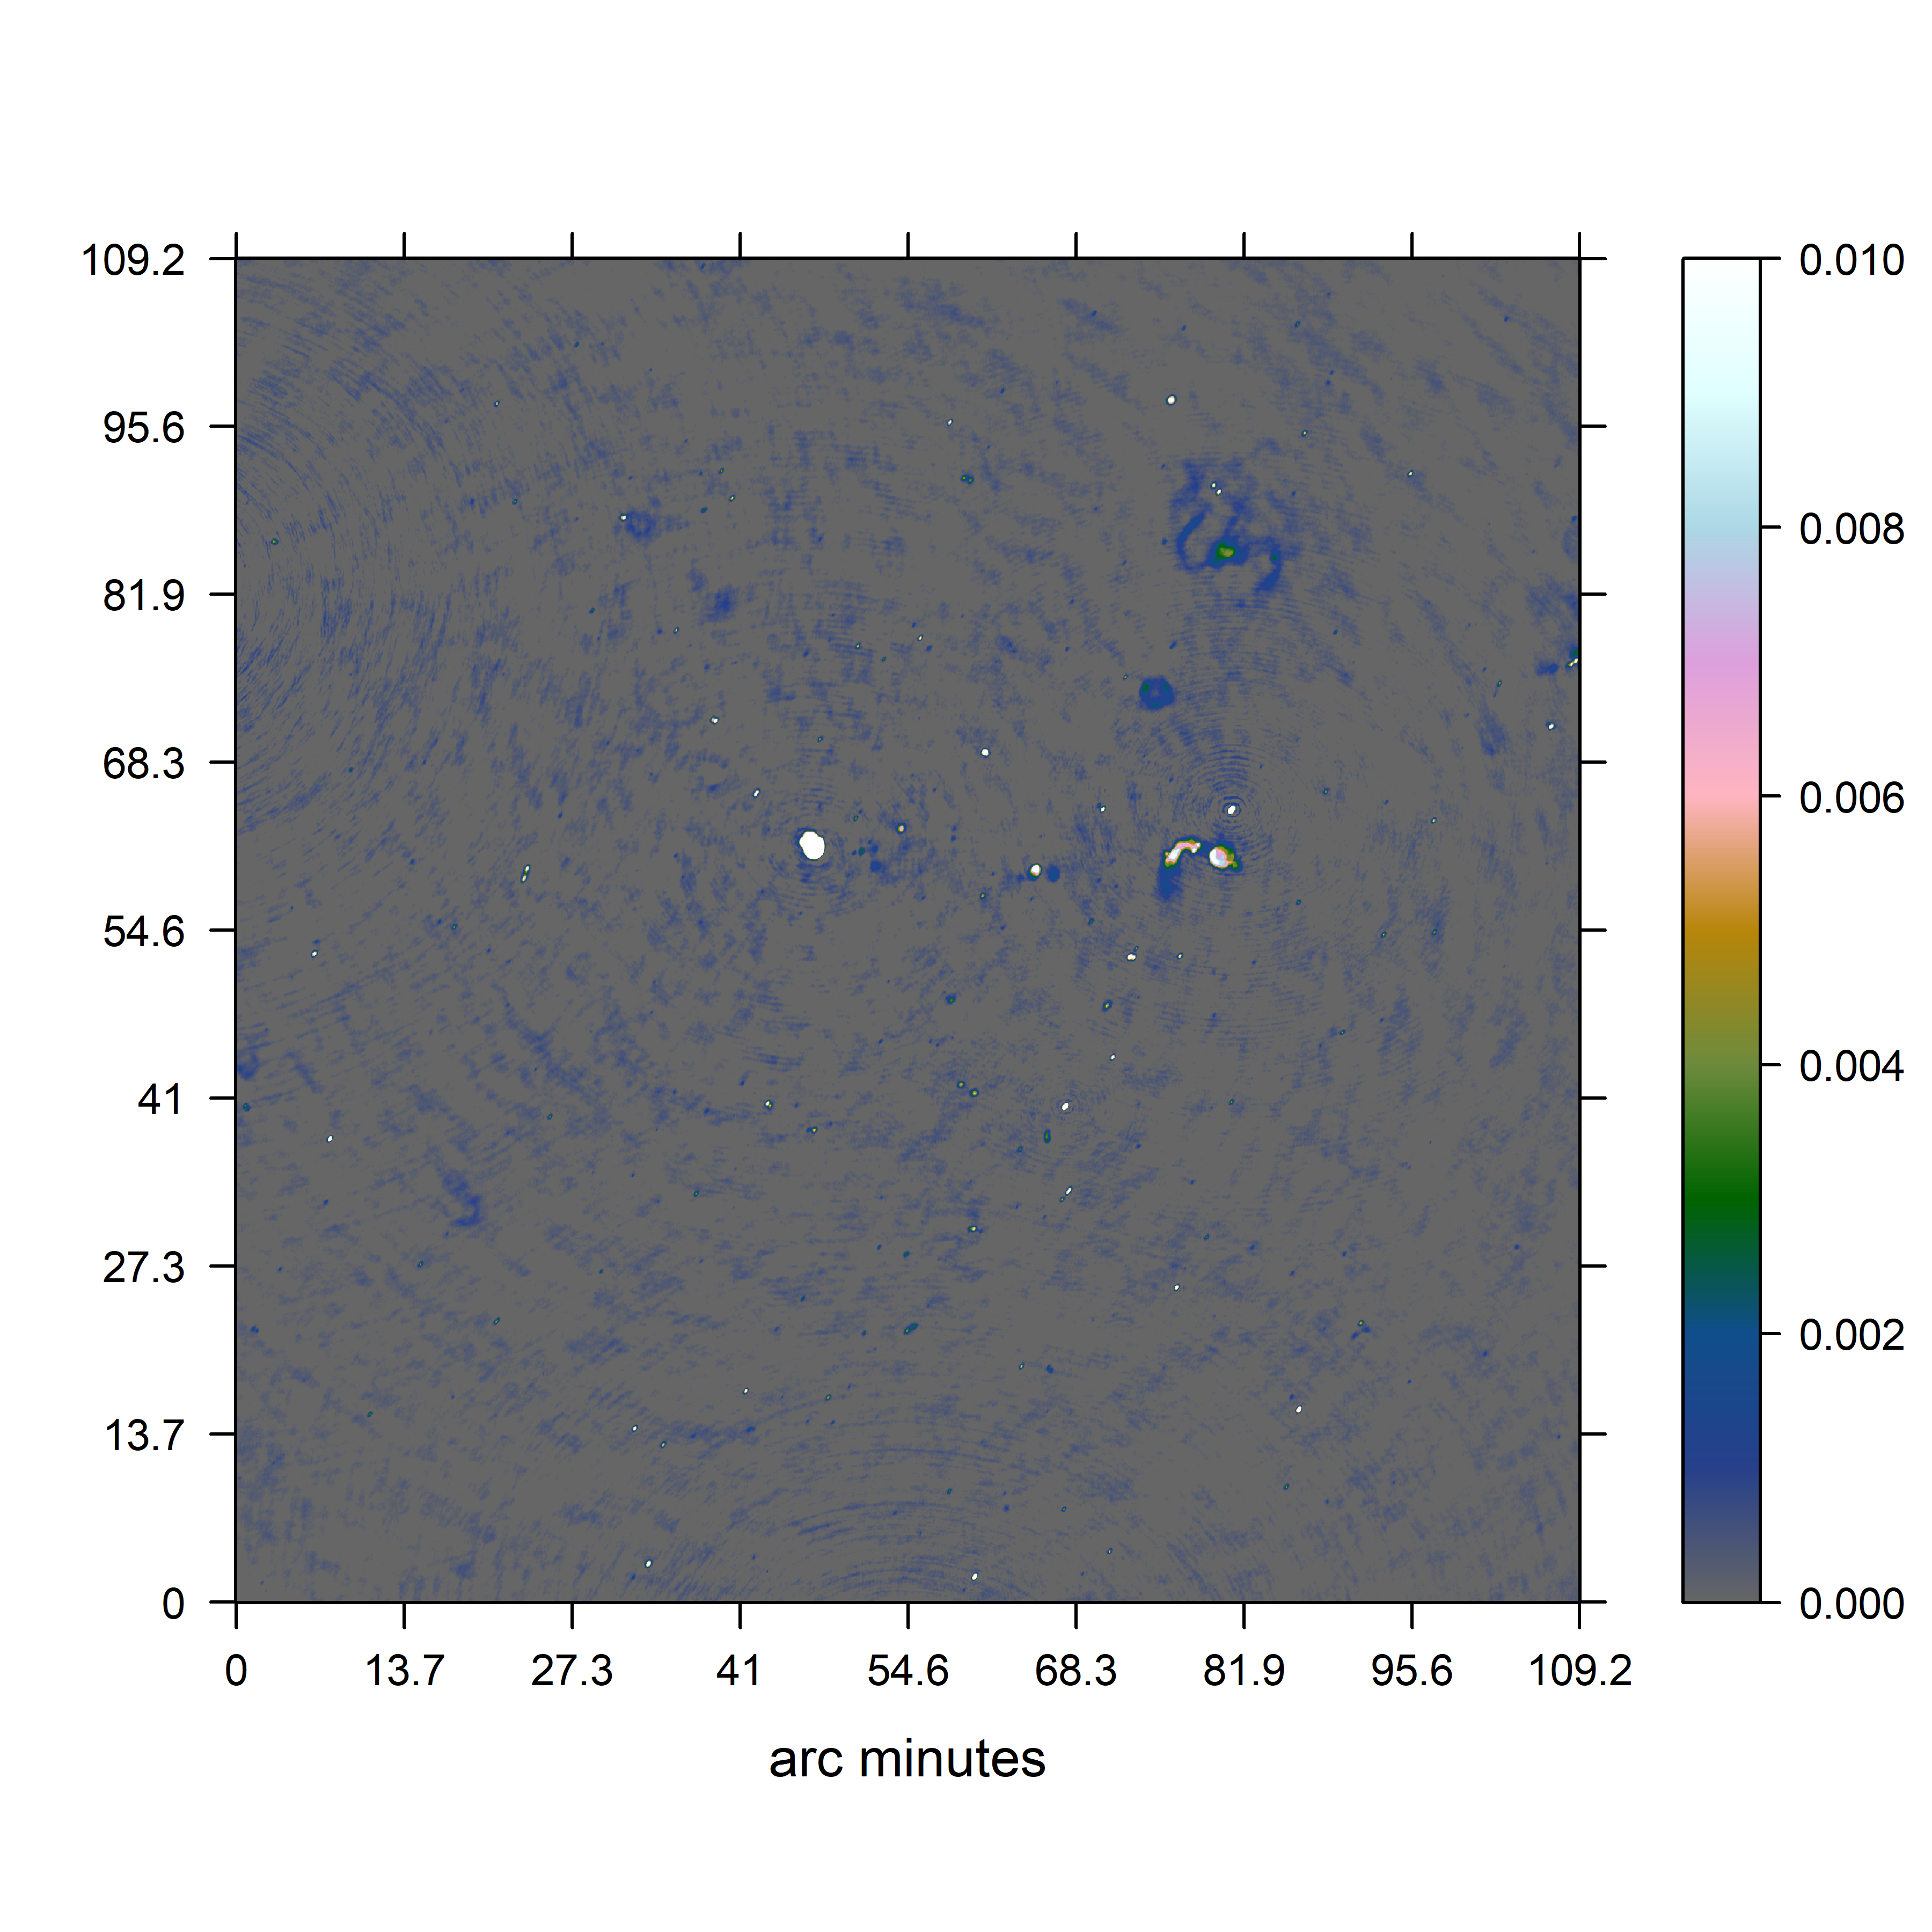
\includegraphics[width=0.6\linewidth]{./chapters/21.scalability/meerkat.png}
	\caption{WSCLEAN Reconstruction of the MeerKAT observation.}
	\label{scale:wsclean}
\end{figure}

For Coordinate Descent's costs, we need an estimate for $J$, $S$ and $I_{CD}$. We set $J=8$, which lets the largest structure span over half the image, enough to capture any large scale structures. For $S$ and $I_{CD}$, we simply use the values from our simulated reconstruction \ref{results:mixed:cd} and set $S=250$ and 
$I_{CD}=10$. This is an under-estimation of the true values. The image \ref{scale:wsclean} shows complex-shaped extended emissions, which likely needs a larger number of starlets for representation than the Gaussian emissions from our simulation. 

When we put all values into our cost functions \eqref{results:cd:omega} and \eqref{results:clean:o}, Coordinate Descent with the direct Fourier transform arrives at 1.9 times the costs of WSCLEAN in the best case scenario. Our approach has not reduced the runtime costs compared to WSCLEAN. But what about Major Cycle Compressed Sensing algorithms? We have not developed a cost function for other Major Cycle approaches, but we can get a very rough estimate by changing $I_{Major}$ of the WSCLEAN cost function. Pratley et al.\cite{pratley2018fast} reported 10 Major Cycles for a Compressed Sensing reconstruction on simulated data. If we plug in 10 Major Cycles for WSCLEAN, Coordinate Descent ends up taking roughly 1.2 times the cost of the Major Cycle algorithm. Mind you these costs are only valid when we can keep all necessary columns of $F$ in memory, eating up 1.1 terabytes\footnote{If we assume 64 bit floating point accuracy for the real and complex values of the Visibilities.} in our case. If not, the columns have to be re-calculated on the fly, increasing the runtime costs by factors. 

The issue with Coordinate Descent's runtime complexity lies in the term $I_{CD} * [S * 4M +\ldots]$ of \eqref{results:cd:omega}, which scales with the "content" of the image $S$, multiplied with the Visibilities. Coordinate Descent cannot afford many iterations nor many non-zero components, because both of these numbers get multiplied together with $M$, the largest number in the problem. With the Major Cycle architecture, WSCLEAN is able to get around this limitation, and scales any content dependent factors on $N$ instead of $M$. 

Indeed, the runtime of our Coordinate Descent algorithm could be improved by using the major cycle architecture, essentially replacing $M$ with $N$ and we arrive at the term $I_{CD} * [S * 4N +\ldots]$. By using the Major Cycle architecture, Coordinate Descent can afford more iterations and more non-zero components in the image for the same runtime complexity. Furthermore $N$ lies on a uniformly sampled grid. We may be able to use the FFT instead of caching columns of $F$, and reduce the memory requirement at the same time.


\subsection{Approximations as key for going large scale}
In this project, we created a new architecture for Compressed Sensing reconstructions. Instead of using the non-uniform FFT approximation, we directly use the relevant columns of the Fourier transform matrix. We showed that the likely-relevant columns can be retrieved with a heuristic, and we can reconstruct images without ever calculating the whole Fourier matrix. This architecture naturally extends to the wide field of view measurement equation \eqref{meerkat:ftsphere}. It can handle the $w$-term explicitly and does not need any approximations. 

We created a proof-of-concept algorithm in this architecture, with Coordinate Descent as the optimizer and starlets as regularization. We exploited the starlet for a greedy heuristic, locating the likely-relevant columns of the Fourier transform matrix. The same heuristic can be used with other regularizations. It locates the likely location of Gaussian-like objects at different scales. As such the same heuristic could be used for a Gaussian mixture model. At this point, it is unclear if the heuristic will eventually converge to the true optimum in theory. In practice, we showed super-resolution performance of Coordinate Descent on simulated MeerKAT data together with accurate total flux modelling compared to CLEAN. 

This is a similar result to other Major Cycle compressed sensing algorithms, which have also shown super-resolved reconstructions compared to CLEAN on real-world observations\cite{dabbech2018cygnus}\cite{girard2015sparse}, but also at a higher runtime cost. The main goal of this project was to find a new architecture which reduces the runtime cost of Compressed Sensing algorithms for large scale reconstructions. In the context of MeerKAT, the estimated runtime costs of CLEAN were still half of the best case estimate of our Coordinate Descent algorithm. Ironically, the runtime costs of Coordinate Descent can be improved by using the Major Cycle architecture instead of the direct Fourier transform and potentially reduce its memory requirement as well.

That does not mean the new architecture cannot beat CLEAN or the Major Cycle. Our architecture scales independently of the image size. The cost effectiveness of the two architectures boils down to the ratio between Visibilities and pixels. For MeerKAT reconstructions, the ratio is skewed towards Visibilities, and the Major Cycle is more cost effective. But if we increase the number of pixels in the reconstruction, we increase the cost-effectiveness of our direct Fourier transform architecture.

%my heuristic

Increasing the number of pixels is only useful to a limit. Decreasing the number of Visibilities however, might yield better results: The large number of Visibilities are virtually guaranteed to have redundant information. A portion of the total runtime is spent on Visibilities, which do not contain any new information for the image. One improvement may be to sub-sample the Visibilities and reconstruct an approximate image from a fraction of the dataset. In this environment, our new architecture may become viable for reducing runtime costs. Indeed, the direct Fourier transform may not be cost effective partly because it does not use approximations. Our architecture calculates the Fourier transform up to the limit of floating-point precision. The Major Cycle on the other hand, uses the non-uniform FFT approximation and stops at the noise limit of the measurements. For our new architecture, introducing back approximations may be the key to reduce runtime costs.

In the future MeerKAT is scheduled to be expanded, posing the reconstruction problem on an even larger scale. Sooner or later, the reconstruction has to be done over a distributed computing infrastructure. In the Major Cycle, single steps like the $w$-correction lend themselves to distributed computing. But designing a Major Cycle algorithm which is highly distributable is an open problem. The simplified architecture of our direct Fourier transform together with Coordinate Descent may have an edge in distributed computing. Coordinate Descent can converge, even when the descent steps are distributed. As it exists in this project, the memory and runtime costs of our approach are too high to be relevant for MeerKAT reconstructions. 

However, if we can decrease the memory and runtime costs with the right approximations, while keeping the distribution properties of Coordinate Descent intact, our approach may become interesting for distributed image reconstructions.








 